\documentclass[aspectratio=169, table, 12pt]{beamer}

\usepackage{colortbl}
\usepackage{xcolor}
\usepackage{listings}
\usepackage{tabularx}
\usepackage{tikz}
\usetikzlibrary{arrows.meta, positioning, calc, fit, shapes.geometric}

\makeatletter
\def\input@path{{../theme/}}
\makeatother
\graphicspath{{../theme/}{../../figures/}}
\usetheme{Pradita}

\definecolor{praditagreen}{RGB}{37, 113, 71}

% Tema membuat garis tabel berwarna putih. Dikembalikan agar tabel terbaca.
\arrayrulecolor{black}
\setlength{\arrayrulewidth}{0.5pt}

% Kolom X rata kiri, dipakai pada tabel dengan kolom X yang sempit, agar
% spasi antarkata tidak meregang.
\newcolumntype{Y}{>{\raggedright\arraybackslash}X}

\lstdefinelanguage{bash}{
  keywords={},
  basicstyle=\ttfamily\scriptsize,
  ndkeywords={cd, curl, python, python3, tsc},
  ndkeywordstyle=\color{purple}\bfseries,
  sensitive=true,
  commentstyle=\color{gray},
  numbers=none,
  breaklines=true,
  frame=lines,
  backgroundcolor=\color{lightgray!10},
  tabsize=2,
  comment=[l]{\#},
  showstringspaces=false
}

\lstdefinelanguage{TypeScript}{
  keywords={const, let, function, return, async, await, try, catch, throw,
            new, if, interface, void, export, import, from, type},
  ndkeywords={Promise, number, string, boolean, Buku, HalamanBuku, Pesanan},
  basicstyle=\ttfamily\scriptsize,
  keywordstyle=\color{blue}\bfseries,
  ndkeywordstyle=\color{purple}\bfseries,
  sensitive=true,
  commentstyle=\color{gray}\itshape,
  stringstyle=\color{red},
  numbers=none,
  breaklines=true,
  frame=lines,
  backgroundcolor=\color{lightgray!10},
  tabsize=2,
  comment=[l]{//},
  morestring=[b]",
  showstringspaces=false
}

% Gaya Python disamakan dengan naskah bab, tanpa nomor baris.
\lstdefinestyle{PythonStyle}{
  language=Python,
  basicstyle=\ttfamily\scriptsize,
  morekeywords={with, as, yield, async, await, match, case},
  keywordstyle=\color{blue}\bfseries,
  emph={jsonschema, json},
  emphstyle=\color{purple}\bfseries,
  commentstyle=\color{gray}\itshape,
  stringstyle=\color{red},
  numbers=none,
  breaklines=true,
  frame=lines,
  backgroundcolor=\color{lightgray!10},
  tabsize=2,
  showstringspaces=false
}

% Kontrak ditampilkan apa adanya, sehingga butuh gaya JSON.
\lstdefinelanguage{json}{
  basicstyle=\ttfamily\scriptsize,
  stringstyle=\color{red},
  commentstyle=\color{gray},
  numbers=none,
  breaklines=true,
  frame=lines,
  backgroundcolor=\color{lightgray!10},
  tabsize=2,
  showstringspaces=false,
  morestring=[b]"
}

\title{\Huge Type Safety, Kontrak API,\\ \vspace{10pt} dan Desain Layanan}
\subtitle{IF140303 - Pengembangan Aplikasi Web}
\author{\textbf{Alfa Yohannis}}

\begin{document}

\frame{\titlepage}

\begin{frame}[fragile]
  \frametitle{Isi Pertemuan}
  \vspace{14pt}
  \begin{columns}[t]
    \column{0.5\textwidth}
    {\small\tableofcontents[sections={1-8}]}

    \column{0.5\textwidth}
    {\small\tableofcontents[sections={9-15}]}
  \end{columns}
\end{frame}

\begin{frame}{\hfill}
  \centering
  \Huge{\textbf{Di mana aturan API disimpan:\\di kontrak, atau di kepala
  penulisnya?}}
\end{frame}

\section{Tujuan dan Kerangka Bahasan}

\begin{frame}{\hfill}
  \centering
  \Huge{\textbf{Tujuan dan Kerangka Bahasan}}
\end{frame}

\begin{frame}{{\Large Tujuan Pembelajaran}}
  \vspace{10pt}
  \begin{itemize}
    \item Memformalkan satu API sebagai kontrak OpenAPI, lalu
          meng-\textit{generate} tipe kliennya dari kontrak itu.
    \item Membedakan validasi \textit{runtime} dari pemeriksaan
          \textit{compile-time}, beserta kesalahan yang ditangkap
          masing-masing.
    \item Memisahkan perubahan kontrak yang aman dari yang merusak klien
          lama, lalu membuktikannya pada server yang berjalan.
  \end{itemize}
\end{frame}

\begin{frame}{{\Large API Tidak Dirancang, Melainkan Tumbuh}}
  \vspace{12pt}
  \begin{itemize}
    \item Satu alamat ditambahkan, satu field disisipkan, satu nama diubah
          karena nama lamanya terasa kurang tepat.
    \item Selama pemakainya penulisnya sendiri, cara itu bekerja. Begitu ada
          klien lain, tiap perubahan menjadi taruhan.
    \item Bab ini memindahkan API dari kebiasaan menjadi kontrak yang dapat
          dibaca mesin.
  \end{itemize}
  \vspace{10pt}
  {\small Demonya satu API katalog berisi 48 buku, dilayani dalam dua versi
  sekaligus, dengan satu \textit{gateway} di depannya.}
\end{frame}

\section{Kontrak sebagai Sumber Kebenaran}

\begin{frame}{\hfill}
  \centering
  \Huge{\textbf{Kontrak sebagai Sumber Kebenaran}}
\end{frame}

\begin{frame}{{\Large Satu Kontrak, Empat Pemakaian}}
  \vspace{4pt}
  \centering
  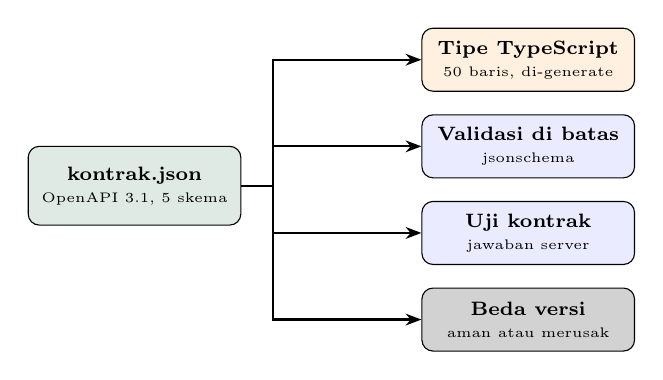
\begin{tikzpicture}[
    font=\scriptsize,
    kotak/.style={draw, rounded corners, minimum height=0.8cm,
                  minimum width=2.7cm, align=center, font=\scriptsize\bfseries},
    panah/.style={-{Stealth[length=2mm]}, thick}
  ]
    \node[kotak, fill=praditagreen!15, minimum height=1.0cm] (kontrak) at (0,0) {kontrak.json\\{\tiny\mdseries OpenAPI 3.1, 5 skema}};
    \node[kotak, fill=orange!12] (tipe) at (5.0,1.6) {Tipe TypeScript\\{\tiny\mdseries 50 baris, di-generate}};
    \node[kotak, fill=blue!8] (validasi) at (5.0,0.5) {Validasi di batas\\{\tiny\mdseries jsonschema}};
    \node[kotak, fill=blue!8] (uji) at (5.0,-0.6) {Uji kontrak\\{\tiny\mdseries jawaban server}};
    \node[kotak, fill=gray!35] (diff) at (5.0,-1.7) {Beda versi\\{\tiny\mdseries aman atau merusak}};

    \draw[panah] (kontrak.east) -- ++(0.4,0) |- (tipe.west);
    \draw[panah] (kontrak.east) -- ++(0.4,0) |- (validasi.west);
    \draw[panah] (kontrak.east) -- ++(0.4,0) |- (uji.west);
    \draw[panah] (kontrak.east) -- ++(0.4,0) |- (diff.west);
  \end{tikzpicture}
  \vspace{2pt}
  {\small Analoginya gambar kerja bangunan: tukang tidak menebak lebar pintu
  dari dinding yang sudah berdiri.}
\end{frame}

\begin{frame}[fragile]{{\Large Dua Baris yang Menentukan Perilakunya}}
  \vspace{2pt}
\begin{lstlisting}[language=json]
"PesananBaru": {
  "type": "object",
  "required": ["id_buku", "jumlah"],
  "additionalProperties": false,
  "properties": {
    "id_buku": { "type": "integer", "minimum": 1 },
    "jumlah": { "type": "integer", "minimum": 1, "maximum": 10 }
  }
}
\end{lstlisting}
  \vspace{2pt}
  {\small \texttt{required} menyebut field yang wajib ada, dan
  \texttt{additionalProperties: false} menolak field yang tidak disebutkan.}
\end{frame}

\section{Validasi di Batas Sistem}

\begin{frame}{\hfill}
  \centering
  \Huge{\textbf{Validasi di Batas Sistem}}
\end{frame}

\begin{frame}[fragile]{{\Large Satu Pemeriksaan di Pintu Masuk}}
  \vspace{2pt}
\begin{lstlisting}[style=PythonStyle]
def periksa_isi(versi, isi):
  try:
    jsonschema.validate(isi, skema(versi, "PesananBaru"))
  except jsonschema.ValidationError as kesalahan:
    return kesalahan.message
  return None
\end{lstlisting}
  \vspace{2pt}
  {\small Panjangnya enam baris, karena aturannya tidak ditulis di sana,
  melainkan dibaca dari kontrak. Sesudah lolos, kode di belakangnya boleh
  memperlakukan isinya sebagai data yang bentuknya pasti.}
\end{frame}

\begin{frame}{{\Large Lima Isi Permintaan, Diukur}}
  \vspace{6pt}
  \centering
  {\footnotesize
  \begin{tabularx}{\textwidth}{Yll}
    \hline
    \textbf{Isi yang dikirim} & \textbf{Status} & \textbf{Alasan dari server} \\
    \hline
    sesuai kontrak & 201 & diterima \\
    \hline
    field wajib \texttt{id\_buku} hilang & 422 & isi tidak sesuai \\
    \hline
    \texttt{id\_buku} bertipe string & 422 & isi tidak sesuai \\
    \hline
    \texttt{jumlah} bernilai 99 & 422 & isi tidak sesuai \\
    \hline
    ada field asing \texttt{catatan} & 422 & isi tidak sesuai \\
    \hline
  \end{tabularx}}
  \vspace{6pt}
  {\small Baris terakhir sering mengejutkan: field asing ditolak, bukan
  diabaikan. Salah tulis nama field ketahuan seketika, dan menambah field
  baru menjadi perubahan kontrak yang harus disengaja.}
\end{frame}

\section{Tipe Hasil Generate}

\begin{frame}{\hfill}
  \centering
  \Huge{\textbf{Tipe Hasil Generate}}
\end{frame}

\begin{frame}{{\Large Runtime lawan Compile-Time}}
  \vspace{6pt}
  \centering
  {\footnotesize
  \begin{tabularx}{\textwidth}{lYY}
    \hline
    \textbf{Hal} & \textbf{Runtime} & \textbf{Compile-time} \\
    \hline
    Yang diperiksa & data yang tiba & kode yang ditulis \\
    \hline
    Kapan & saat permintaan dilayani & sebelum program jalan \\
    \hline
    Menangkap & isi permintaan yang salah & pemakaian field yang tidak ada \\
    \hline
    Tidak menangkap & salah tulis di kode klien & data dari klien lain \\
    \hline
    Pada demo ini & \texttt{jsonschema} di server & \texttt{tsc --strict} di klien \\
    \hline
  \end{tabularx}}
  \vspace{6pt}
  {\small Keduanya diperlukan, dan keduanya menangkap hal yang berbeda.}
\end{frame}

\begin{frame}[fragile]{{\Large Tipe Datang dari Kontrak, Bukan dari Tangan}}
  \vspace{2pt}
\begin{lstlisting}[language=TypeScript]
export interface HalamanBuku {
  item: Buku[];
  halaman: number;
  per_halaman: number;
  total: number;
  berikutnya?: string;
}

export interface Pesanan {
  id: string;
  id_buku: number;
  jumlah: number;
  status: "diterima" | "diproses";
}
\end{lstlisting}
  \vspace{2pt}
  {\small Tanda tanya datang dari daftar \texttt{required}, dan daftar nilai
  \texttt{status} datang dari \texttt{enum} di kontrak.}
\end{frame}

\begin{frame}[fragile]{{\Large Perubahan Kontrak Tertangkap Compiler}}
  \vspace{2pt}
\begin{lstlisting}[language=bash]
../chapter06/node_modules/.bin/tsc --noEmit --strict --ignoreConfig \
  pakai-tipe-salah.ts

# Keluarannya:
# pakai-tipe-salah.ts(15,15): error TS2339: Property 'harga' does not
# exist on type 'Buku'.
\end{lstlisting}
  \vspace{4pt}
  {\small Pada kontrak versi 2, field \texttt{harga} berganti nama menjadi
  \texttt{harga\_rupiah}. Klien lama ditolak sebelum programnya jalan, bukan
  oleh pengguna.}
\end{frame}

\section{Model Error, Pagination, dan Filtering}

\begin{frame}{\hfill}
  \centering
  \Huge{\textbf{Model Error, Pagination,\\dan Filtering}}
\end{frame}

\begin{frame}{{\Large Satu Bentuk Error untuk Semua Alamat}}
  \vspace{10pt}
  \begin{itemize}
    \item Bentuknya Problem Details:
          \texttt{application/problem+json} dengan \texttt{type},
          \texttt{title}, \texttt{status}, dan \texttt{detail}.
    \item Isi \texttt{detail} berasal dari validator, sehingga klien tahu
          field mana yang salah tanpa menebak.
    \item \textit{Pagination} dan \textit{filtering} ditulis di kontrak
          sebagai parameter, lengkap dengan batasnya.
  \end{itemize}
  \vspace{8pt}
  {\small Pada katalog 48 buku: \texttt{/v1/buku} menjawab 10 item dan total
  48, \texttt{?halaman=2} menjawab halaman kedua, dan
  \texttt{?per\_halaman=99} dijawab 422 karena batas kontraknya 50.}
\end{frame}

\section{Idempotency}

\begin{frame}{\hfill}
  \centering
  \Huge{\textbf{Idempotency}}
\end{frame}

\begin{frame}[fragile]{{\Large Satu Kunci, Satu Pesanan}}
  \vspace{2pt}
\begin{lstlisting}[style=PythonStyle]
  sidik = json.dumps(isi, sort_keys=True)
  if kunci in IDEMPOTENSI:
    sidik_lama, id_pesanan = IDEMPOTENSI[kunci]
    if sidik_lama != sidik:
      return None, 409
    return PESANAN[id_pesanan], 200
\end{lstlisting}
  \vspace{2pt}
  {\small Analoginya nomor setoran di loket: ketika mahasiswa datang lagi
  dengan nomor yang sama karena struknya hilang, petugas mencetak ulang
  struknya, bukan mencatat setoran kedua.}
\end{frame}

\begin{frame}{{\Large Tiga Permintaan, Diukur}}
  \vspace{6pt}
  \centering
  {\footnotesize
  \begin{tabularx}{\textwidth}{Yll}
    \hline
    \textbf{Permintaan} & \textbf{Status} & \textbf{Hasil} \\
    \hline
    kunci baru & 201 & pesanan \texttt{psn-0002} dibuat \\
    \hline
    kunci sama, isi sama & 200 & \texttt{psn-0002} dikembalikan \\
    \hline
    kunci sama, isi beda & 409 & ditolak, kunci sudah dipakai \\
    \hline
  \end{tabularx}}
  \vspace{6pt}
  {\small Perhatikan baris kedua: 200, bukan 201, karena tidak ada yang
  dibuat. Selisih satu angka itu membedakan "pesanan sudah masuk" dari
  "pesanan masuk dua kali".}
\end{frame}

\section{Kompatibilitas dan Versioning}

\begin{frame}{\hfill}
  \centering
  \Huge{\textbf{Kompatibilitas dan Versioning}}
\end{frame}

\begin{frame}{{\Large Lima Perubahan, Dinamai Mesin}}
  \vspace{6pt}
  \centering
  {\footnotesize
  \begin{tabularx}{\textwidth}{Yl}
    \hline
    \textbf{Perubahan v1 ke v2} & \textbf{Akibat} \\
    \hline
    \texttt{Buku.harga} wajib dihapus & merusak klien lama \\
    \hline
    \texttt{Buku.harga\_rupiah} wajib ditambah & merusak klien lama \\
    \hline
    \texttt{Buku.penerbit} opsional ditambah & aman \\
    \hline
    \texttt{Pesanan.status} enum menerima \texttt{dibatalkan} & merusak klien lama \\
    \hline
    \texttt{PesananBaru.jumlah} batas naik ke 20 & aman bagi klien lama \\
    \hline
  \end{tabularx}}
  \vspace{6pt}
  {\small Baris terakhir dibaca dua arah: batas yang dilonggarkan aman bagi
  klien lama, tetapi klien v2 yang memesan 15 ditolak 422 oleh v1.}
\end{frame}

\begin{frame}{{\Large Server Menjawab 200, Klien Tetap Rusak}}
  \vspace{6pt}
  \centering
  {\footnotesize
  \begin{tabularx}{\textwidth}{Yll}
    \hline
    \textbf{Yang diuji} & \textbf{Status} & \textbf{Hasil} \\
    \hline
    klien v1 membaca \texttt{/v1/buku} & 200 & jalan \\
    \hline
    klien v1 membaca \texttt{/v2/buku} & 200 & gagal, \texttt{harga} tidak ada \\
    \hline
    klien v2 memesan 15 ke \texttt{/v2} & 201 & diterima \\
    \hline
    klien v2 memesan 15 ke \texttt{/v1} & 422 & isi tidak sesuai \\
    \hline
  \end{tabularx}}
  \vspace{6pt}
  {\small Baris kedua memuat pelajaran terpentingnya: servernya tidak salah
  sedikit pun, yang rusak kesepakatannya. Kerusakan itu hanya terlihat bila
  ada yang memvalidasi jawaban terhadap kontrak lama.}
\end{frame}

\section{Rate Limiting dan API Gateway}

\begin{frame}{\hfill}
  \centering
  \Huge{\textbf{Rate Limiting dan API Gateway}}
\end{frame}

\begin{frame}{{\Large Token Bucket di Depan Aplikasi}}
  \vspace{4pt}
  \centering
  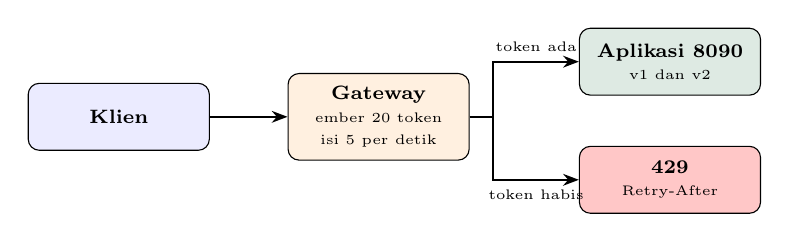
\begin{tikzpicture}[
    font=\scriptsize,
    kotak/.style={draw, rounded corners, minimum height=0.85cm,
                  minimum width=2.3cm, align=center, font=\scriptsize\bfseries},
    panah/.style={-{Stealth[length=2mm]}, thick}
  ]
    \node[kotak, fill=blue!8] (klien) at (0,0) {Klien};
    \node[kotak, fill=orange!12, minimum height=1.1cm] (ember) at (3.3,0) {Gateway\\{\tiny\mdseries ember 20 token}\\{\tiny\mdseries isi 5 per detik}};
    \node[kotak, fill=praditagreen!15] (aplikasi) at (7.0,0.7) {Aplikasi 8090\\{\tiny\mdseries v1 dan v2}};
    \node[kotak, fill=red!22] (tolak) at (7.0,-0.8) {429\\{\tiny\mdseries Retry-After}};

    \draw[panah] (klien) -- (ember);
    \draw[panah] (ember.east) -- ++(0.3,0) |- node[font=\tiny, above, pos=0.75] {token ada} (aplikasi.west);
    \draw[panah] (ember.east) -- ++(0.3,0) |- node[font=\tiny, below, pos=0.75] {token habis} (tolak.west);
  \end{tikzpicture}
  \vspace{2pt}
  {\small Analoginya kupon fotokopi: jatahnya diisi berkala, boleh dipakai
  sekaligus, dan begitu habis harus menunggu pengisian berikutnya.}
\end{frame}

\begin{frame}{{\Large Angkanya Dapat Dihitung Sebelum Diukur}}
  \vspace{6pt}
  \centering
  {\footnotesize
  \begin{tabularx}{\textwidth}{Yllll}
    \hline
    \textbf{Tahap} & \textbf{200} & \textbf{429} & \textbf{Retry-After} & \textbf{Lama} \\
    \hline
    30 permintaan sekaligus & 20 & 10 & 0,19 s & 0,02 s \\
    \hline
    setelah menunggu 2 detik & 10 & 20 & 0,16 s & 0,02 s \\
    \hline
    klien lain, ember sendiri & 20 & 10 & 0,19 s & 0,02 s \\
    \hline
  \end{tabularx}}
  \vspace{6pt}
  {\small Baris pertama melayani 20 karena embernya berisi 20 token. Baris
  kedua melayani 10, karena 2 detik mengisi $2 \times 5$ token. Baris ketiga
  melayani 20 lagi karena embernya milik klien lain, bukan milik sistem.}
\end{frame}

\section{Gaya API}

\begin{frame}{\hfill}
  \centering
  \Huge{\textbf{Gaya API: REST, GraphQL, dan RPC}}
\end{frame}

\begin{frame}{{\Large Tiga Gaya dan Tradeoff-nya}}
  \vspace{6pt}
  \centering
  {\footnotesize
  \begin{tabularx}{\textwidth}{lYYY}
    \hline
    \textbf{Hal} & \textbf{REST} & \textbf{GraphQL} & \textbf{RPC} \\
    \hline
    Bentuk & sumber daya beralamat & satu alamat, \textit{query} klien & daftar fungsi \\
    \hline
    Kontrak & OpenAPI & skema GraphQL & \textit{protocol buffer} \\
    \hline
    Cache HTTP & langsung dapat dipakai & perlu usaha tambahan & umumnya tidak \\
    \hline
    Ambil data berlebih & sering & jarang & tergantung fungsinya \\
    \hline
    Cocok untuk & API publik & layar dengan kebutuhan beragam & layanan ke layanan \\
    \hline
  \end{tabularx}}
  \vspace{6pt}
  {\small Pilihan gayanya jarang menjadi penentu mutu API. Yang menentukan
  sama pada ketiganya: kontrak yang dapat dibaca mesin, bentuk \textit{error}
  yang seragam, batas laju yang jelas, dan perubahan versi yang tidak
  diam-diam.}
\end{frame}

\section{Persiapan Latihan}

\begin{frame}{\hfill}
  \centering
  \Huge{\textbf{Persiapan Latihan}}
\end{frame}

\begin{frame}[fragile]{{\Large Dua Perintah}}
  \vspace{2pt}
\begin{lstlisting}[language=bash]
cd sources/chapter12
python3 aplikasi.py &
python3 gateway.py &

# Keluarannya:
# Melayani di http://127.0.0.1:8090/v1/buku dengan 48 buku
# Gateway di http://127.0.0.1:8091/ dengan ember 20 token
\end{lstlisting}
  \vspace{4pt}
  {\small Latihan membutuhkan Python 3 beserta \texttt{jsonschema}, dan
  \texttt{tsc} yang sudah terpasang di Bab 6. Tanpa Docker dan tanpa
  pemasangan npm baru.}
\end{frame}

\section{Latihan 1: Generate Tipe}

\begin{frame}{\hfill}
  \centering
  \Huge{\textbf{Latihan 1:\\Generate Tipe dari Kontrak}}
\end{frame}

\begin{frame}[fragile]{{\Large Meng-generate lalu Memeriksanya}}
  \vspace{2pt}
\begin{lstlisting}[language=bash]
python3 buat_tipe.py kontrak.json tipe-katalog.ts
python3 buat_tipe.py kontrak-v2.json tipe-katalog-v2.ts
../chapter06/node_modules/.bin/tsc --noEmit -p tsconfig.json

# Keluarannya:
# 5 skema dan 2 jalur di-generate menjadi tipe-katalog.ts
# 5 skema dan 2 jalur di-generate menjadi tipe-katalog-v2.ts
\end{lstlisting}
  \vspace{2pt}
  {\small Lalu tambahkan satu field opsional pada skema \texttt{Buku},
  jalankan ulang generatornya, dan catat perubahan file tipenya.}
\end{frame}

\section{Latihan 2: Validasi dan Idempotensi}

\begin{frame}{\hfill}
  \centering
  \Huge{\textbf{Latihan 2:\\Validasi dan Idempotensi}}
\end{frame}

\begin{frame}[fragile]{{\Large Sebelas Baris Hasil Pengujian}}
  \vspace{2pt}
\begin{lstlisting}[language=bash]
python3 uji-kontrak.py

# Keluarannya:
#   Yang diuji                   Status  Hasil
#   sesuai kontrak                  201  sesuai, diterima
#   field asing                     422  sesuai, isi tidak sesuai
#   kunci baru                      201  pesanan psn-0002 dibuat
#   kunci sama, isi sama            200  pesanan psn-0002 dikembalikan
#   kunci sama, isi beda            409  kunci idempotensi dipakai ulang
\end{lstlisting}
  \vspace{2pt}
  {\small Nyalakan ulang aplikasinya lebih dahulu, agar nomor pesanannya
  dimulai dari awal.}
\end{frame}

\section{Latihan 3: Kompatibilitas}

\begin{frame}{\hfill}
  \centering
  \Huge{\textbf{Latihan 3:\\Kompatibilitas Antarversi}}
\end{frame}

\begin{frame}[fragile]{{\Large Membandingkan Kontrak lalu Mengujinya}}
  \vspace{2pt}
\begin{lstlisting}[language=bash]
python3 uji-kompatibilitas.py

# Keluarannya:
#   Perubahan kontrak v1 ke v2                     Akibat
#   Buku.harga wajib dihapus                       merusak klien lama
#   Buku.penerbit opsional ditambah                aman
#   PesananBaru.jumlah batas naik ke 20            aman bagi klien lama
#
#   klien v1 membaca /v2/buku             200  gagal: 'harga' is required
#   klien v2 memesan 15 ke /v1            422  isi tidak sesuai
\end{lstlisting}
  \vspace{2pt}
  {\small Lalu ganti nama satu field wajib di kontrak v2, dan catat berapa
  baris "merusak klien lama" yang muncul.}
\end{frame}

\section{Latihan 4: Batas Laju}

\begin{frame}{\hfill}
  \centering
  \Huge{\textbf{Latihan 4:\\Batas Laju di Gateway}}
\end{frame}

\begin{frame}[fragile]{{\Large Mengukur Lonjakan dan Pengisian Ulang}}
  \vspace{2pt}
\begin{lstlisting}[language=bash]
python3 ukur-gateway.py

# Keluarannya:
#   Tahap                            200   429  Retry-After  Lama detik
#   30 permintaan sekaligus           20    10         0.19        0.02
#   setelah menunggu 2 detik          10    20         0.16        0.02
#   klien lain, ember sendiri         20    10         0.19        0.02
\end{lstlisting}
  \vspace{2pt}
  {\small Hitung sendiri angka tahap kedua dari lama menunggu dan laju
  pengisiannya, lalu ubah \texttt{KAPASITAS\_EMBER} menjadi 5 dan ukur
  sekali lagi.}
\end{frame}

\section{Ringkasan}

\begin{frame}{\hfill}
  \centering
  \Huge{\textbf{Ringkasan}}
\end{frame}

\begin{frame}{{\Large Ringkasan}}
  \vspace{8pt}
  \begin{itemize}
    \item Satu dokumen OpenAPI berisi 5 skema dan 2 jalur dipakai empat kali:
          50 baris tipe, validasi isi, validasi jawaban, dan perbandingan
          versi.
    \item Validasi \textit{runtime} menolak 4 dari 5 isi yang diuji dengan
          422. Pemeriksaan \textit{compile-time} menolak klien yang membaca
          field lama dengan TS2339.
    \item Idempotensi mengubah pengiriman ulang menjadi hal biasa: kunci sama
          dan isi sama dijawab 200 beserta pesanan yang sudah ada, kunci sama
          dan isi beda dijawab 409.
    \item Kompatibilitas dapat diperiksa mesin. Klien v1 membaca jawaban v2
          dengan status 200 tetapi gagal memakainya.
    \item \textit{Token bucket} melayani 20 lalu menolak 10, dan menunggu 2
          detik memulihkan tepat 10 token.
  \end{itemize}
\end{frame}

\end{document}
